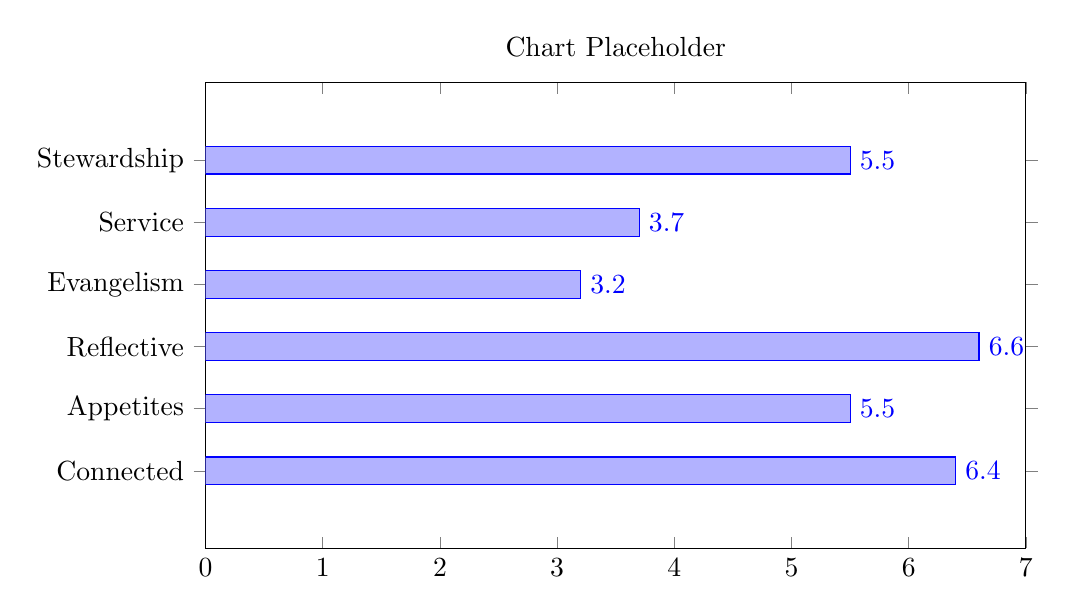
\begin{tikzpicture}
  \begin{axis}[
    title=Chart Placeholder,
    xbar, xmin=0, xmax=7,
    width=12cm,
    height=7.5cm,
    enlarge y limits=0.25,
    symbolic y coords={Connected,Appetites,Reflective,Evangelism,Service,Stewardship},
    ytick=data,
    nodes near coords,
    nodes near coords align={horizontal},
    ]
    \addplot coordinates {
      (6.4,Connected)
      (5.5,Appetites)
      (6.6,Reflective)
      (3.2,Evangelism)
      (3.7,Service)
      (5.5,Stewardship)
    };
  \end{axis}
\end{tikzpicture}
